% Chapter 3

\chapter{Travail réalisé} % Main chapter title

\label{Chapter3} % For referencing the chapter elsewhere, use \ref{Chapter3} 

%----------------------------------------------------------------------------------------

\section{Génération d'une méta-donnée (RP,AA)}

Pour réaliser une métadonnée nous avons lancé la commande suivante :

\begin{tcolorbox}
    user@poky:~\$ yocto-layer create-layer your\_layer\_name
\end{tcolorbox}

Elle nous assiste lors de la génération d’une grande partie de l’architecture standardisée
commune aux metas. \medskip 

Nous avons ensuite comparé notre meta à la meta-skeleton, le squelette de base
permettant de doter notre système d’exploitation d’un programme helloworld. \medskip 

Nous aurions préféré partir de la commande ci-dessous seulement celle-ci n’est
accessible avant la version 2.4 du projet.

\begin{tcolorbox}
    user@poky:~\$ bitbake-layer create-layer your\_layer\_name
\end{tcolorbox}

Nous rajoutons cette meta à la liste des objets à compiler par la commande suivante.

\begin{tcolorbox}
    user@poky:~\$ bitbake-layer add-layer your\_layer\_name
\end{tcolorbox}

Après utilisation voici à quoi la meta ressemble depuis l’interface de développement atom.

\begin{figure}[!htb]
    \centering
    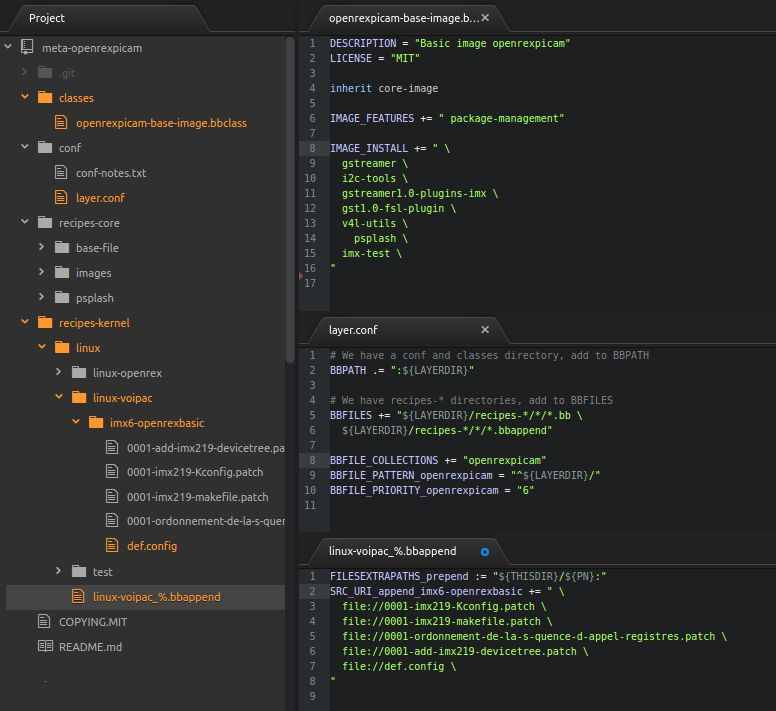
\includegraphics[trim={0cm 0cm 0cm 0cm},clip,scale=0.31]{Figures/architecture.png}
    \decoRule
    \caption{Architecture d'une méta-donnée} \label{fig:architecture}
\end{figure} 

Au début de la création de notre métadonnée nous souhaitions pouvoir reconstituer notre
espace de travail aisément et cela est possible grâce aux deux dépôts
fsl-community-bsp-platform et fsl-community-bsp-base de Freescale. Cependant il est
nécessaire de les modifier afin qu’ils correspondent à aux fichiers nécessaires à notre
meta-donnée. \medskip 

Le dépôt fsl-community-bsp-platform contient un fichier “default.xml” que l’on appelle un
fichier manifest, celui-ci permet de définir tous les dépôts contenant les fichiers et dossiers
nécessaires à la création de notre image Yocto. \medskip 

Le second dépôt fsl-community-bsp-data créera notre fichier “bblayers.conf”
avec toutes les métadonnées nécessaires à la compilation ainsi que le fichier
“setup-environment” qui concevra notre fichier local.conf.

\subsection{fsl-community-bsp-platform (RP)}

Nous avons repris le “default.xml” utilisé par Frescale incluant un kernel 4.1
\href{http://git.freescale.com/git/cgit.cgi/imx/fsl-arm-yocto-bsp.git/tree/default.xml?h=imx-4.1-krogoth}
{(sur ce lien)}

Cela a permis de connaître les dépôts ainsi que leurs branches afin de réaliser notre
propre fichier manifest. Nous avons rajouté les liens vers notre méta-donnée ainsi que
notre dépôt fsl-community-bsp-data grâce à ces deux lignes : \medskip

\begin{lstlisting}
    <remote fetch="git://github.com/petit-romain" name="romain"/>
    <remote fetch="git://github.com/Alanaitali" name="equipe"/>    
\end{lstlisting}

On a donné l’ordre de récupérer le fichier “setup-environment” permettant de sourcer notre
environnement de travail en le plaçant dans le dossier sources/base : \medskip 

\begin{lstlisting}
    <project remote="romain" revision="master" name="fsl-community-bsp-base" path="sources/base">
        <copyfile dest="setup-environment" src="setup-environment"/>
    </project>
\end{lstlisting}

Enfin on précise la branche sur laquelle nous développons notre meta ainsi que son
emplacement dans notre dossier de travail (sources/meta-openrexpicam) :

\begin{lstlisting}
    <project remote="equipe" revision="develop/porting" path="sources/meta-openrexpicam"/>
\end{lstlisting}

\subsection{fsl-community-bsp-data (RP)}

Ce dépôt recopiera automatiquement notre fichier “bblayers.conf” puisqu’il
contient le contenu du fichier : 

\begin{lstlisting}
    BBLAYERS = " \
    ${BSPDIR}/sources/poky/meta \
    ${BSPDIR}/sources/poky/meta-Yocto \
    \
    ${BSPDIR}/sources/meta-openembedded/meta-oe \
    ${BSPDIR}/sources/meta-openembedded/meta-multimedia \
    \
    ${BSPDIR}/sources/meta-fsl-arm \
    ${BSPDIR}/sources/meta-fsl-arm-extra \
    ${BSPDIR}/sources/meta-fsl-demos \
    \
    ${BSPDIR}/sources/meta-openrexpicam \
    "
    BBLAYERS += "${BSPDIR}/sources/meta-fsl-arm-voipac"
\end{lstlisting}

Pour le fichier “setup-environment”, nous n’avions rien à modifier cependant nous avons
ajouté une signature ainsi que les images compilables de notre méta-donnée :

\begin{lstlisting}
    Welcome to our project !
    You can now run 'bitbake <target>'
    Common targets are :
        - openrexpicam-base-image
    Signed-off-by: Alan Ait-Ali, Romain Petit, Clément Ailloud & Martin Laporte
\end{lstlisting}

\section{Génération d'un OS (RP,ML,AA)}

\subsection{Préparation de l'environnement (RP,AA)}

Grâce à l’environnement de travail Yocto nous avons pu rapidement mettre en place un
système d’exploitation fonctionnel sur la cible Openrex. En effet les équipes de Voipac et
Fedevel ont mis à disposition le support de la carte (BSP) afin que la distribution
GNU/Linux maintenue par Freescale pour les processeurs imx6 fonctionne sur les
Openrex. L’ensemble de sources fsl-community-bsp supporte donc la carte
Openrex-imx6q. Cette officialité permet, une fois les sources correctement téléchargées et
ordonnées, de compiler une image par la commande :

\begin{tcolorbox}
    MACHINE=imx6s-openrex bitbake core-image-base
\end{tcolorbox}

\subsection{Préparation de notre meta-donnée (RP,AA)}

Le projet Yocto permet aussi d’améliorer l’image générée. Cette amélioration suit le principe des
codes ouverts à l’amélioration et fermés aux modifications. En effet comme représenté sur la
figure \ref{fig:recette}, lors de la compilation des recettes (100 Mo) nécessaires à la core-image-base, le
programme bitbake a puisé dans des sources distantes pour composer un dossier de sources à compiler. 
Grâce à celles-ci bitbake forme un répertoire général des sources du noyau (18Go), bitbake compile 
ensuite la core-image-base et la place dans :  \medskip

\$BUILDDIR/tmp/deploy/images/{NOM\_DE\_L’IMAGE:imx6-openrexbasic} \medskip

Mais pour modifier cette image il n’y a pas besoin de toucher aux recettes des
meta-données initiales (100Mo sur la figure \ref{fig:recette}). Pour modifier l’image on intervient
d'abord au niveau du dossier des sources (18Go) on apporte nos améliorations. De ces
modifications on réalise un patch différenciant l’état d’origine et l’état actuel des fichiers
voulus. Enfin on vient placer ce patch dans notre propre meta (1Mo) à côté des
meta-données originales. En visionnant cette meta et les patchs qui s’y trouvent on
versionne donc l’ensemble du projet depuis l’état d’origine fixé par la communauté
freescale.

\begin{figure}[!htb]
    \centering
    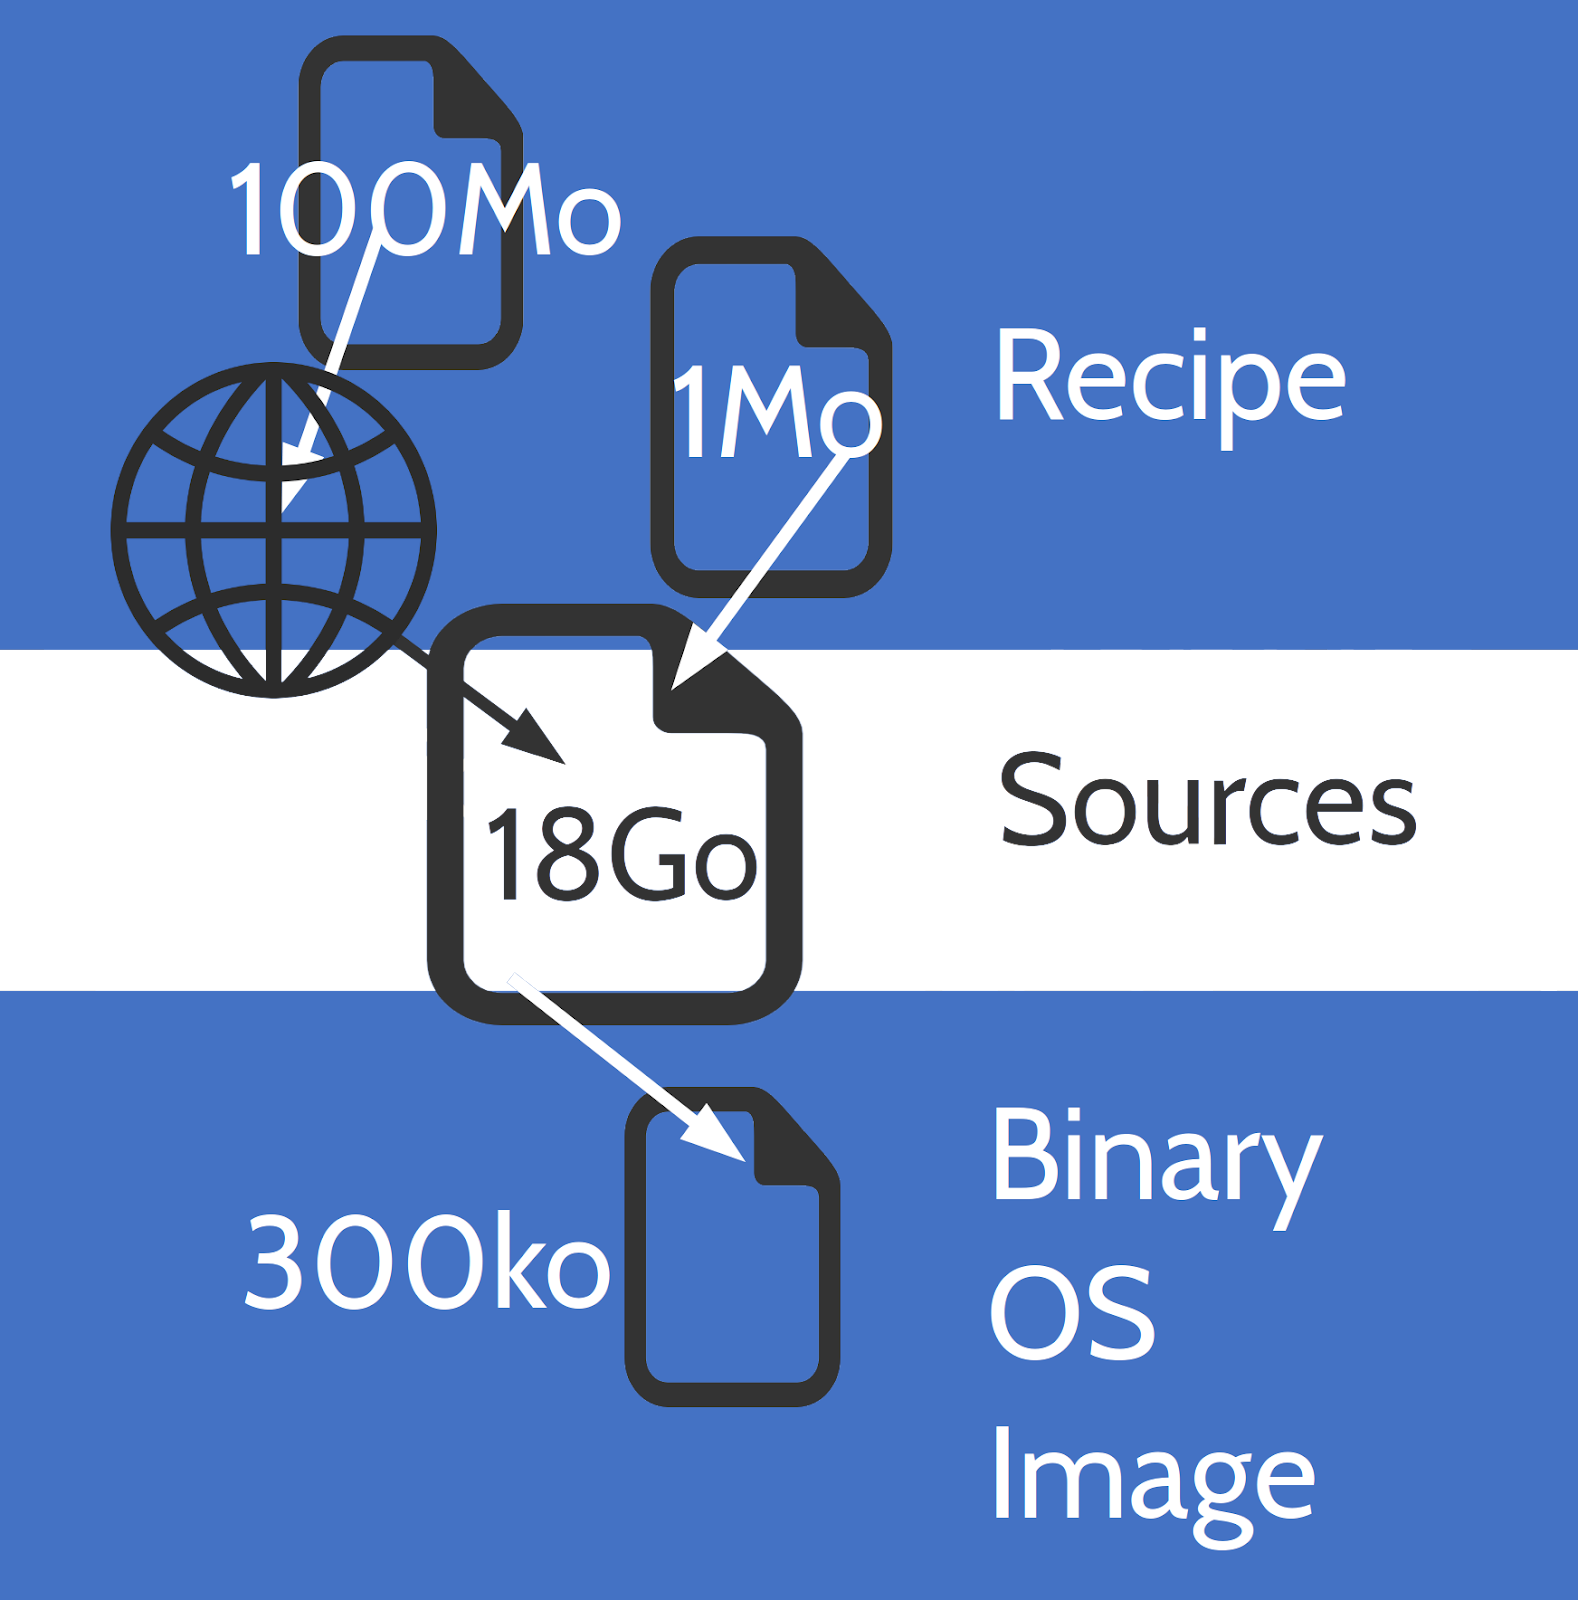
\includegraphics[trim={0cm 0cm 0cm 0cm},clip,scale=0.1]{Figures/recette.png}
    \decoRule
    \caption{Architecture d'une recette} \label{fig:recette}
\end{figure} 

\section{Implémentation de code dans le BSP (AA)}

Le coeur du projet vise à ajouter du code dans le bsp déjà existant, notamment au sein du
kernel. Pour ce faire nous modifions le dossier de compilation (18Gb ci-dessus). Comme
son nom l’indique, /git/ est versionné par git et nous permet de tirer un patch de nos
modifications. \medskip

Ensuite, on applique des patchs modifiant les sources du kernel provenant
du git de voipac ou fedevel. le patch généré est inclu aux sources de notre recette
linux-voipac\_\%.bbappend. La recette s'ajoutera à la fin de la recette linux-voipac lors de
sa prise en compte par bitbake. \medskip

La recette linux-voipac\_\%.bbappend a pour rôle de surcharger la recette se trouvant dans
la meta-fsl-arm-voipac. Elle porte le même nom que la recette a surcharger suivi d’un \_\%
qui permet de s’affranchir de la version. \medskip

Dans l’extrait ci-dessous on peut voir que la recette utilise les sources du git voipac.

\subsection{Extrait de linux-voipac-4.1.bb}

\begin{lstlisting}
SRCBRANCH = "4.1-2.0.x-imx-rex"
LOCALVERSION = "-Yocto"
SRCREV = "ab5923c9613a97ede4da92a933842e771283d463"
KERNEL_SRC ?= "git://github.com/voipac/linux-fslc.git;protocol=git"
SRC_URI = "${KERNEL_SRC};branch=${SRCBRANCH} file://defconfig"
\end{lstlisting}

Notre recette permet d’ajouter les fichiers se trouvant dans imx6-openrexbasic et inscrit
dans la recette comme on le voit ci-dessous.

\subsection{Extrait de linux-voipac\_ \%.bbappend}

\begin{lstlisting}
    FILESEXTRAPATHS_prepend := "${THISDIR}/${PN}:"
    SRC_URI_append_imx6-openrexbasic += " \
        file://0001-imx219.patch \
        file://defconfig \
    "
\end{lstlisting}

Quand nous modifions le code du dossier de compilation, le patch se réfère à l’état dans
lequel la communauté des bsp freescale l’a laissé. Or dans le fichier
\$BUILDDIR/conf/bblayer.conf notre meta-openrexpicam est placée directement en suivant
des meta nécessaires pour atteindre l’état laissé par freescale. Nous sommes donc sûrs
que le patch généré est cohérent avec l’arborescence de compilation sur laquelle bitbake
l’appliquera.

\section{Implémentation des supports de compilation (AA)}

Ajouter une nouvelle caméra a notre BSP, demande la création d’un driver. Pour qu’il soit
utilisable il nous faut signaler au compilateur que nous voulons ajouter à notre kernel le
support pour la caméra. Pour paramétrer la compilation on passe par l’outil menuconfig
qui permet 3 options :

\begin{itemize}
    \item[-] compilation du driver et chargement en module
    \item[-] compilation du driver et chargement en statique
    \item[-] pas de compilation du driver
\end{itemize}

Les fichiers qui permettent de paramétrer le menuconfig sont situés au même endroit que
les fichiers source.c des pilotes sous le nom de Kconfig.

L’ajout de notre caméra dans menuconfig se fait par le code suivant :

\begin{lstlisting}
    config MXC_CAMERA_IMX219_MIPI
    tristate "Sony imx219 camera support using mipi (raspicam v2)"
    depends on !VIDEO_MXC_EMMA_CAMERA && I2C
\end{lstlisting}

\begin{itemize}
    \item[depends on : ] Définit les modules à activer pour que l’option soit visible
    \item[tristate : ] Définit l’affichage dans le menuconfi
    \item[Config : ] Définit le nom de la variable de compilation
\end{itemize}

\begin{figure}[!htb]
    \centering
    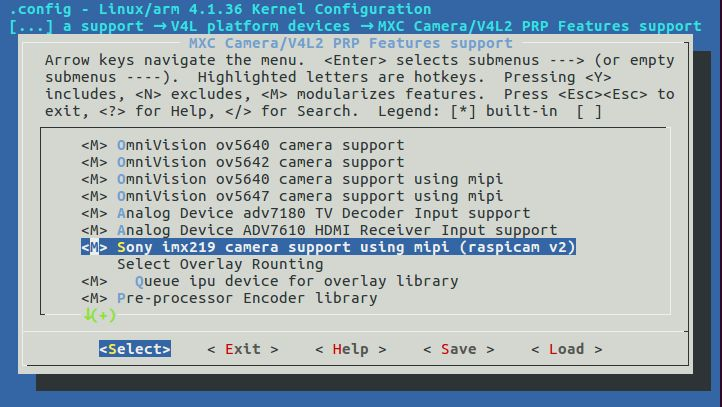
\includegraphics[trim={0cm 0cm 0cm 0cm},clip,scale=0.4]{Figures/menuconfig.png}
    \decoRule
    \caption{Driver dans le menuconfig} \label{fig:menucfg}
\end{figure}

Sur la figure ci-dessus on peut remarquer un M juste devant les drivers, cela signifie qu’ils
sont compilés en module. Nous avons choisi cette option afin de pouvoir décharger
(rmmod) et recharger (modprobe) le driver sans devoir redémarrer le kernel.
Le résultat du menuconfig est un fichier texte .config
(\$BUILDDIR/tmp/work/imx6\_openrexbasic-poky-linux-gnueabi/linux-voipac/4.1-r0/build/ex
emple.config) ou généralement defconfig. Dans l’extrait du defconfig ci-dessous on peut
observer que l’ajout et le chargement en module du pilote a été pris en compte.

\begin{lstlisting}
    CONFIG_VIDEO_MXC_IPU_CAMERA=y
    CONFIG_MXC_CAMERA_OV5640=m
    CONFIG_MXC_CAMERA_OV5642=m
    CONFIG_MXC_CAMERA_OV5640_MIPI=m
    CONFIG_MXC_CAMERA_OV5647_MIPI_INT=m
    CONFIG_MXC_TVIN_ADV7180=m
    CONFIG_MXC_TVIN_ADV7610=m
    CONFIG_MXC_CAMERA_IMX219_MIPI=m
    CONFIG_MXC_IPU_DEVICE_QUEUE_SDC=m
    CONFIG_MXC_IPU_PRP_ENC=m
    CONFIG_MXC_IPU_CSI_ENC=m
\end{lstlisting}

\begin{itemize}
    \item[-] CONFIG\_MXC\_CAMERA\_IMX219\_MIPI : Objet du kernel
    \item[-] m : Ordre de compilation et d'installation en module
\end{itemize}

Le menuconfig permet de configurer la compilation, mais il n’est pas directement lié à
celle-ci, c’est le Makefile qui se charge de relier les informations contenues dans le .config
au compilateur. Comme le Kconfig, le Makefile se trouve dans le répertoire des sources :
\$BUILDDIR/tmp/work/{imx6\_openrexbasic-poky-linux-gnueabi/{recette}/4.1-r0/git/drivers/media/{Selon le driver}

Selon le driver, ses sources peuvent prolonger ce chemin vers “platform/mxc/capture/” ou
“/i2c/.”. Le nom de la recette, lui dépends du kernel compilé. La recette “linux-openrex” est
utilisée pour les kernels v3 et “linux-voipac” pour les kernels v4.

\begin{lstlisting}
    +imx219_camera_mipi-objs := imx219_mipi.o
    +obj-$(CONFIG_MXC_CAMERA_IMX219_MIPI) += imx219_camera_mipi.o
\end{lstlisting}

\begin{itemize}
    \item[-] imx219\_camera\_mi-objs : nom du fichier .c à compiler
    \item[-] CONFIG\_MXC\_CAMERA\_IMX219\_MIPI : variable de compilation fourni par le .config
    \item[-] imx219\_camera\_mipi.o nom du driver compilé
\end{itemize}

Au lancement de bitbake le driver pourra alors être compilé et chargé par le kernel.

\section{Utilsation de drivers existants (ML,CA,RP,AA)}

\subsection{Présentation d'un driver (ML)}

Un driver Linux est un programme binaire qui s’exécute dans le kernel-space. Un driver
utilise les ABI kernel pour interagir avec son environnement. Le code d’un driver s’appuie
donc sur les API kernel. Dans le cas du système d’exploitation linux, celles-ci sont
rédigées en langage c. C’est pourquoi il est nécessaire que le compilateur du driver
compile parfaitement le langage c. Dans notre cas comme dans la majorité, le driver sera
écrit en c. Une particularité des codes de driver provient de l’absence de main(), celui-ci
est remplacé par des fonctions init() et exit(). Init() permet le chargement du driver dans le
kernel. Si le driver est compilé en statique, il est chargé (linked and locked) au démarrage
et exit() est exécuté lors de l’extinction du système. Si le driver est compilé en module ce
sont les fonctions insmod et rmmod qui appelleront les init et exit du fichier “.ko”

\subsection{Utilisation de l'existant (RP,AA)}

Dans un premier temps, n’étant pas habitués à manipuler des drivers, nous avons
cherché à utiliser des sources en croisant les architectures requises. Pour agir dans notre meta,
nous avons eu recours à une série de patchs comme montrés ci-dessous.

\begin{figure}[!htb]
    \centering
    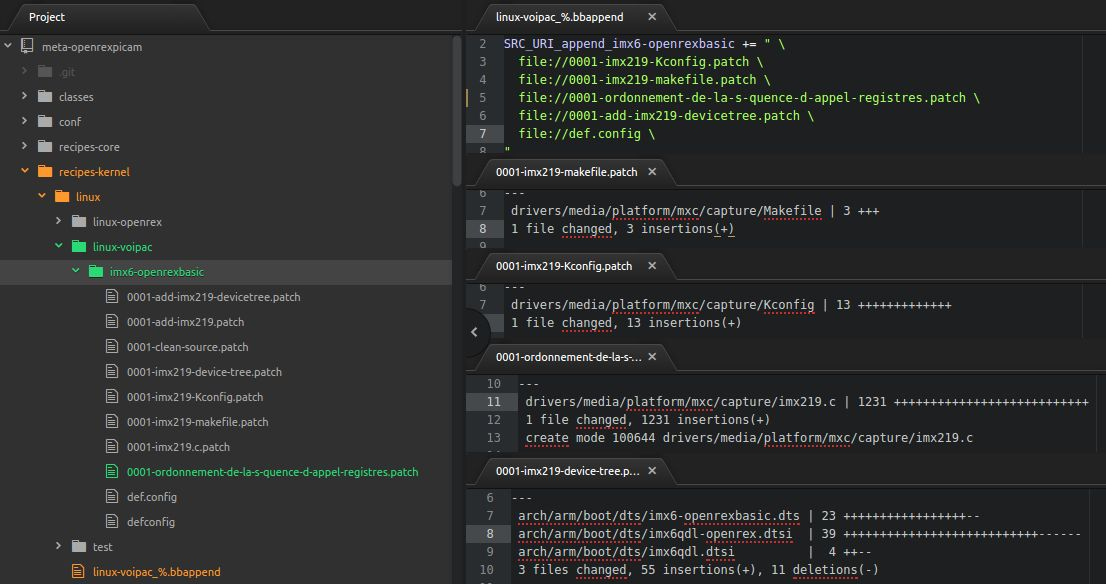
\includegraphics[trim={0cm 0cm 0cm 0cm},clip,scale=0.35]{Figures/patchs.png}
    \decoRule
    \caption{Patchs du kernel 3.14} \label{fig:patchs}
\end{figure} 

\subsubsection{Compilation par SDK (ML,CA)}

Dans un premier temps, nous nous doutions qu’il y aurait des erreurs de compilation.
Nous avons préféré décorréler les erreurs de compilation de nos propres erreurs. Nous
avons alors essayé de compiler ces fichiers, en dehors de la meta depuis la
cross-toolchain générée par Yocto. Nous utilisons la variable \$CC sélectionnant le cross
compilateur, cette variable est affectée lorsque l’on “source” le sdk généré par :

\begin{tcolorbox}
    \#génération du sdk
    bitbake openrexpicam-base-image -c populate\_sdk
    \#environement du sdk
    source /opt/poky/2.0.3/environment-setup-cortexa9hf-vfp-neon-poky-linux-gnueabi
    \#aperçu de CC
    CC=arm-poky-linux-gnueabi-gcc -march=armv7-a -marm -mthumb-interwork -mfloat-abi=hard -mfpu=neon
    -mtune=cortex-a9 –sysroot=/opt/poky/2.0.3/sysroots/cortexa9hf-vfp-neon-poky-linux-gnueabi
    \#première compilation « out-of-tree »
    \$CC imx219.c
\end{tcolorbox}

Cette compilation fait appel à des bibliothèques contenues dans les arborescences de
compilation de différentes recettes. 

\begin{tcolorbox}
    BUILDDIR=/home/diag/workspaceThales/YOCTO/fsl-community-bsp/build-imx6rex.com
    IMX6S\_DIR=\$BUILDDIR/tmp/work/imx6s\_openrex-poky-linux-gnueabi
    \#libs linux/*.h
    DIRLINUX=\$IMX6S\_DIR/linux-openrex/3.14-r0/git/include
    DIRLINUX2=\$IMX6S\_DIR/u-boot-openrex/v2015.10+gitAUTOINC+7d8ddd7de7-r0/git/include
    DIRLINUX3=\$IMX6S\_DIR/core-image-minimal/1.0-r0/sdk/image/opt/poky/2.0.3/sysroots/cortexa9hf-vfp-neon
    -poky-linux-gnueabi/usr/include
    \#libs asm/*.h
    DIRASM=\$BUILDDIR/tmp/work/x86\_64-nativesdk-pokysdk-linux/nativesdk-linux-libc-headers/4.1-r0/linux-4.1
    /arch/arm/include/
    DIRASM2=\$IMX6S\_DIR/linux-openrex/3.14-r0/build/arch/arm/include/generated
    DIRASM3=\$IMX6S\_DIR/u-boot-openrex/v2015.10+gitAUTOINC+7d8ddd7de7-r0/git/arch/arm/include/
    \#nouvelle commande de compilation « out of tree »
    \$CC imx219.c -I\$DIRLINUX -I\$DIRASM -I\$DIRASM2 -I\$DIRLINUX2 -I\$DIRLINUX3 -I\$DIRASM3
\end{tcolorbox}

Nous avons inclus 6 dossiers de bibliothèques en option puis les nouvelles dépendances
étaient inexistantes dans le dossier contenant l’arborescence de compilation. Donc nous
nous sommes mis à chercher une autre solution. Après avoir parlé à notre professeur de
Linux embarqué des soucis de compilation que nous rencontrions nous nous sommes mis
à compiler le driver en ajoutant ses sources dans l’arborescence (in-tree).

\subsubsection{Compatilation out-of-tree (ML,CA)}

Pour cette première compilation de code source dans Yocto nous avons tout d'abord
rédigé une recette comme on aurait rédigé un makefile. Un intérêt est de pouvoir compiler
nos sources sans avoir à recompiler le kernel entier. Seulement cette méthode ne résout
pas le problème de gestion des dépendances. En effet même si Yocto compile avec la
même configuration le kernel et ce module, Yocto interprètera les recettes comme deux
compilations différentes et les exécutera dans des répertoires dissociés. les includes du
module seront incapables de trouver plus automatiquement que de manière out-of-tree
leurs bibliothèques kernel (linux/example.h).

\begin{figure}[!htb]
    \centering
    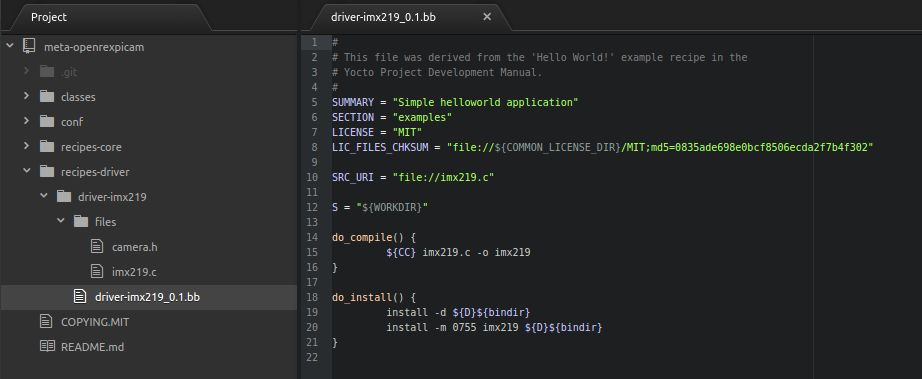
\includegraphics[trim={0cm 0cm 0cm 0cm},clip,scale=0.35]{Figures/outtree.png}
    \decoRule
    \caption{Arborescence de la compilation out-of-tree} \label{fig:outtree}
\end{figure} 

\subsubsection{Compatilation in-tree (ML,AA)}

La compilation de ces sources a été effectuée in-tree sur la version v3.14 du kernel
linux-openrex (branche develop/Smart). La compilation ayant fonctionné, elle a été testée
et déclarée image non bootable. Comme à ce moment là les sources de type chromium os
étaient plus avancées, cette piste fut abandonnée.

\subsection{imx219 - Hummingboard (AA)}

\subsubsection{Origine des sources}

Comme nous n’avions pas encore manipulé un driver par son code source nous sommes
rapidement allés demander des conseils aux professeurs renseignés. Principalement M
P.-J. Texier qui nous gardera à l’oeil le long de ce projet. Dans un mail à notre équipe M
Texier nous a proposé de s’inspirer du driver disponible à l’adresse suivante. Il s’agit du git
“Russell King's ARM Linux kernel tree” mais surtout d’un patch qui ajoute le driver
d’imx219 et configure le makefile et kconfig pour sa compilation. L’intérêt principal étant la
plateforme cible, une “hummingboard” portant un soc imx6dl, différent mais proche de
notre imx6s.
De plus sur ce même kernel tree, on peut trouver les fichiers device-tree correspondants
au driver pour la configuration en question (
\href{http://git.armlinux.org.uk/cgit/linux-arm.git/commit/?h=csi-v6&id=e3f847cd37b007d55b76282414bfcf13abb8fc9a}
{source}, 
\href{http://git.armlinux.org.uk/cgit/linux-arm.git/commit/?h=csi-v6&id=4bd8e1231a2e6eca6a65b565176ea9722611c8dd}
{dts}).

Lors des rapports intermédiaires présentés à l’équipe de Thales nous parlions de ces
sources sous le nom de “solution 3”

\subsubsection{Compilation in-tree (RP)}

Sur les conseils de M Texier, nous n’avons pas cherché à réaliser de compilation
out-of-tree. Nous avons donc directement porté le driver sur notre carte ainsi que les
structures device-tree.

\subsection{imx219 - Nvidia-Tegra Chromium-Os (CA,AA)}

Chromium OS est “un système d’exploitation visant à renforcer la sécurité des utilisateurs qui
passent une majorité de leur temps sur le web”. Concrètement cet os est un système GNU/Linux et
correspond à la branche en développement libre de “Google Chrome os”. Développé par par une filiale
de Google, cet os est entre autre maintenu par Nvidia sur ses processeurs Tegra. Ceux-ci
sont destinés à des applications dans le domaine des smartphones ; ces processeurs
respectent très probablement à la lettre les contraintes MIPI.

\subsubsection{Origine des sources}

Le driver en question provient du git officiel de chromium os de nvidia pour les cartes
tegra, sur le kernel 3.14. il est accessible à ce
\href{https://chromium.googlesource.com/chromiumos/third_party/kernel/+/factory-ryu-6486.14.B-chromeos-3.14/drivers/media/}{lien} .
Lors des rapports intermédiaires présentés à l’équipe de Thales nous parlions de ces
sources sous le nom de “solution 2”.

\subsubsection{Compatibilité avec le device tree}

Lorsque l’on essayait de charger le driver imx219, nous obtenions l’erreur suivante

\begin{tcolorbox}
    imx219 1-0064: IMX219: missing platform data !
\end{tcolorbox}

Après analyse du driver l’erreur provient de la fonction probe du driver. Cette erreur est
survenue dû à une mauvaise compatibilité entre le driver imx219 et le gestionnaire I2C,
pour cela nous avons ajouté une compatibilité avec le device-tree de cette façon :

\begin{lstlisting}
    static const struct of_device_id imx219_of_match [] =
    {
        { . compatible = " sony , imx219 " , . data = 0 } ,
        {}
    };
    MODULE_DEVICE_TABLE ( of , imx219_of_match ) ;
\end{lstlisting}

Ensuite nous avons créé notre propre structure I2C pour l’imx219 afin d’implémenter la
compatibilité entre le driver et l’I2C de cette manière :

\begin{lstlisting}
    static struct i2c_driver imx219_i2c_driver =
    {
        . driver =
            {
                . name = " imx219 " ,
                . of_match_table = of_match_ptr(imx219_of_match) ,
            },
        . probe = imx219_probe ,
        . remove = imx219_remove ,
        . id_table = imx219_id ,
    };
\end{lstlisting}

De plus nous avons enlevé la condition qui nous procurait l’erreur précédente afin de
tester dans un premier temps si la compilation s'effectuait correctement :

\begin{lstlisting}
    if (! ssdd)
    {
        dev_err(& client->dev, "IMX219:missing platform data !\ n");
        return -EINVAL ;
    }
\end{lstlisting}

Après avoir modifié le driver nous obtenons une nouvelle erreur :

\begin{tcolorbox}
    imx219 1-0064: Error -19 getting clock \\
    i2c 1-0064: Driver imx219 requests probe deferral
\end{tcolorbox}

\begin{lstlisting}
    if (! ssdd)
    {
        dev_err(& client->dev, "IMX219:missing platform data !\ n");
        return -EINVAL ;
    }
\end{lstlisting}

Nous avons repris la même stratégie que précédemment en enlevant la condition
générant l’erreur :

\begin{lstlisting}
    if(IS_ERR(priv->clk))
    {
        dev_info(&client->dev,"Error %ld getting clock \ n",
        PTR_ERR(priv->clk));
        return -EPROBE_DEFER ;
    }
\end{lstlisting}

Enfin la capture d’écran ci-dessous permet de justifier que le module se charge bien au
lancement de notre OS :

\begin{tcolorbox}
    root@openrexpicam:~\# i2cdetect -y 1 \\
        \hspace{0.8cm}0\hspace{0.3cm}1\hspace{0.3cm}2\hspace{0.3cm}3\hspace{0.3cm}4\hspace{0.3cm}5
        \hspace{0.3cm}6\hspace{0.3cm}7\hspace{0.3cm}8\hspace{0.3cm}9\hspace{0.3cm}a\hspace{0.3cm}b
        \hspace{0.3cm}c\hspace{0.3cm}d\hspace{0.3cm}e\hspace{0.3cm}f \\
    00: - - - - - - - - - - - - - - - - - - - - - - - - - - - - - - - - \\
    10: 10  - - - - - - - - - - - - - - - - - - - - - - - - - - - - - - \\
    20: - - - - - - - - - - - - - - - - - - - - - - - - - - - - - - - - \\
    30: - - - - - - - - - - - - - - - - - - - - - - - - - - - - - - - - \\
    40: 40  - - - - - - - - - - - - - - 48  - - - - - - - - - - - - - - \\
    50: uu  - - - - - - - - - - - - - - - - - - - - - - - - - - - - - - \\
    60: - - - - - - - - - - uu  - - - - - - - - - - - - - - - - - - - - \\
    70: - - - - - - - - - - - - - - - - - - - - - - - - - - - - - - - - \\
    
    root@openrexpicam:~\# lsmod \\
    Module                      \hspace{2.5cm}Size        \hspace{2cm}Used by\\
    mxc\_v4l2\_capture          \hspace{0.8cm}25109       \hspace{1.75cm}0 \\
    ipu\_bg\_overlay\_sdc       \hspace{0.5cm}5242        \hspace{1.9cm}1 mxc\_v4l2\_capture\\
    ipu\_still                  \hspace{2.5cm}2312        \hspace{1.95cm}1 mxc\_v4l2\_capture\\
    ipu\_prp\_end               \hspace{1.65cm}5872       \hspace{1.95cm}1 mxc\_v4l2\_capture\\
    ipu\_csi\_enc               \hspace{1.9cm}3743        \hspace{1.95cm}1 mxc\_v4l2\_capture\\
    v4l2\_int\_device           \hspace{1.23cm}2913       \hspace{1.95cm}2 ipu\_csi\_enc, mxc\_v4l2\_capture\\
    ipu\_fg\_overlay\_sdc       \hspace{0.55cm}6068       \hspace{1.95cm}1 mxc\_v4l2\_capture\\
    imx219                      \hspace{2.7cm}7716        \hspace{1.95cm}1 \\
    mxc\_dcic                   \hspace{2.3cm}6543        \hspace{2cm}0\\
    galcore                     \hspace{2.65cm}225000     \hspace{1.65cm}0\\
    evbug                       \hspace{2.8cm}1871        \hspace{2.05cm}0\\
\end{tcolorbox}

Une fois ceci effectué nous voulions essayer de corriger les instructions conditionnelles de
sécurité générant les erreurs afin de pouvoir charger correctement le driver. Une fois le
driver chargé, nous n’avons pas réussi à effectuer la liaison entre v4l2 et le driver imx219.
Par manque de temps et de connaissances sur l’environnement v4l2, nous nous sommes
tous concentré sur la nouvelle solution proposé par Thalès qui leur semblait plus
pertinente.

\subsection{imx219 - Raspberry Pi v2 (AA)}

\subsubsection{Origine des sources}
En premier lieu nous sommes partis des sources reçues dans les premiers
mails. Ce driver lie le processeur Allwinner A80 (ARM Cortex-A15/A7) du sbc Raspberry Pi à un
composant pilote vidéo imx219. Ces deux fichiers Linux V4L2 Driver (imx219.c et
camera.h) onts été rédigés par “Chomoly“ et sont téléchargeables à cette 
\href{https://www.raspberrypi.org/forums/viewtopic.php?f=43&t=162722}{adrese}. \medskip

Lors des rapports intermédiaires présentés à l’équipe de Thales nous parlions de ces
sources sous le nom de “solution 1”. \medskip

Chronologiquement, ces fichiers sources ont été la première piste explorée c’est pourquoi
leur compilation n’a pas été immédiatement réussie. Nous avons essayé d’obtenir un
module binaire par trois manières. D’abord, une compilation grâce à un sdk yocto, puis
une compilation out-of-tree, externe à la recette du kernel et nous sommes presque
parvenus à nos fins avec une compilation in-tree. Ci-dessous, la description des pratiques
à éviter pour le projet d’un driver.

\subsubsection{Portage du BSP Voipac sur un kernel 4.14 (AA,RP)}

Lors de nos recherches pour les compilations ci-dessous, nous avons trouvé un driver
imx219 fonctionnel sur un kernel 4.14 donc l’idée était de porter notre méta-donnée vers
un kernel 4.14 afin de réutiliser le driver sur cette version de kernel.
Nous sommes partis de la même structure que les versions de kernel 3.14 et 4.1 qui
contient un dossier avec le defconfig et les différents patchs nécessaires à la compilation
ainsi qu’un fichier .bb.

\begin{tcolorbox}
    user@poky~\$ : tree sources/meta-fsl-arm-voipac/recipes-kernel/linux \\
    |\_\_linux-voipac-3.14 \\
    |\_\_\_\_\_defconfig \\
    |\_\_linux-voipac\_3.14.bb \\
    |\_\_linux-voipac-4.1 \\
    |\_\_\_\_\_defconfig \\
    |\_\_linux-voipac\_4.1.bb \\
    |\_\_linux-voipac-4.14 \\
    |\_\_\_\_\_0001-imx6s-6q-add-initial-support.patch \\
    |\_\_\_\_\_defconfig \\
    |\_\_linux-voipac\_4.14.bb \\
\end{tcolorbox}

Ensuite nous avons modifié la recette du kernel 4.1 dans une nouvelle recette pour un
kernel 4.14 avec les modifications suivantes :

\begin{lstlisting}
    SRCBRANCH = "4.14.x+fslc"
    LOCALVERSION = "-Yocto"
    SRCREV = "${AUTOREV}"
    KERNEL_SRC ?= "git://github.com/Freescale/linux-fslc.git;protocol=git"
\end{lstlisting}

Cependant lors de la phase de boot nous obtenons l’erreur suivante :

\begin{tcolorbox}
    reading boot-imx6-openrexbasic.scr \\
    ** Unable to read file boot-imx6-openrexbasic.scr **
\end{tcolorbox}

Nous pouvons conclure qu’il y a une incompatibilité entre le bootloader et le kernel que
nous avons modifié. Pour que notre image puisse se lancer correctement, il est nécessaire
de modifier le bootloader.

\section{Développement d'un driver (AA,RP,CA,ML)}

Des caméras utilisant le MIPI CSI sont implémentées de base dans le kernel, l’OV5640 en
est un bon exemple. Il s’agit d’un capteur vidéo développé par Omnivision qui se trouve
être ressemblant à l’imx219 au niveau du protocole de communication avec la carte mère.
Le pilote déjà implémenté servira alors de base pour la création d’un driver imx219.

\subsection{Organisation d'un driver MIPI/CSI (AA)}

On dénombre 3 sections principale dans ce genre de pilote :
La première contient en majeure partie du code lié au fonctionnement du composant. On y
retrouve des structures contenant les registres à configurer, les différents modes
d’acquisitions d’image tel que la résolution, la gestion des régulateurs, les signaux de
démarrage et d’extinction, et d’autres caractéristiques. Cette section étant spécifique au
périphérique, c’est ici que seront modifiés un grand nombre de fonction. En effet les
registres et les séquences d’initialisation sont différentes entre les deux composants, il est
donc nécessaire de les adapter.
La deuxième est constituée de fonctions de contrôle et d’initialisation propres à V4L2.
Elles permettent d’enregistrer et d’utiliser l’imx219 en tant qu’appareil V4L2.
La dernière partie est relative à la gestion de la communication i2c, les fonctions
classiques d’un périphérique i2c sont présentes tel que ov5640\_probe, ov5640\_remove,
ov5640\_init et ov5640\_clean sans oublier la structure reliant les fonctions au système
ov5640\_i2c\_driver.

\subsubsection{Intégration au device tree (AA,CA)}

Le device tree est un sous-ensemble composé de plusieurs fichiers configurant toutes les
liaisons entre le matériel et le logiciel. Il permet d’utiliser des drivers conçus pour linux. On
le retrouve dans la partition boot qui est accessible en lecture/écriture, cela permet de le
modifier facilement. Nous pouvons donc tester les drivers de façon rapide et efficace.

La configuration du driver imx219 :

\textbf{extrait de openrexbasic.dts}

\begin{lstlisting}
    &i2c2 {
/* Raspberry Pi camera rev 2.1 */
camera: imx219_mipi@64{
compatible = "sony,imx219";reg = <0x64>;
clocks = <&clks IMX6QDL_CLK_DUMMY>;
clock-names = "csi_mclk";
DOVDD-supply = <&reg_1p8v>;
AVDD-supply = <&reg_2p8v>;
DVDD-supply = <&reg_1p5v>;
pwn-gpios = <&gpio7 6 GPIO_ACTIVE_HIGH>;
csi_id = <1>;
mclk = <24000000>;
mclk_source = <0>;
pinctrl-names = "default";
pinctrl-0 = <&pinctrl_imx219>;
};
\end{lstlisting}

\textbf{extrait de imx6qdl-openrex.dtsi}

\begin{lstlisting}
    &mipi_csi 
    {
        ipu_id = <0>;
        csi_id = <1>;
        v_channel = <1>;
        lanes = <2>;
        mipi_dphy_clk = <0x28>;
        status = "okay";
    };

    pinctrl_imx219: imx219_grp
    {
        fsl,pins = <MX6QDL_PAD_SD3_DAT2__GPIO7_IO06 0x00017059>;
    };
\end{lstlisting}

l’extrait ci-dessus représente la déclaration du driver imx219 dans le
device tree.

\begin{itemize}
    \item[-]compatible = “sony,imx219” : correspond au nom associé
    dans la structure imx219\_i2c\_driver sous la variable .name
    \item[-]reg =<0x64> : correspond à l’adresse i2c du périphérique
    \item[-] clocks = <\&clks IMX6QDL\_CLK\_DUMMY> : lien vers l'horloge à utiliser
    \item[-] clock-names = "csi\_mclk" : nom de l’horloge
    \item[-] pwn-gpios = <\&gpio76GPIO\_ACTIVE\_HIGH> : gpio qui contrôle l’allumage
    \item[-] csi\_id = <1> : identifiant vers la structure CSI
    \item[-] mclk = <24000000> : fréquence de l’horloge
    \item[-] mclk\_source = <0> : source de l’horloge en accord avec la structure v4l2\_cap\_1
    \item[-] pinctrl-0 = <\&pinctrl\_imx219> : lien vers la déclaration des gpios
\end{itemize}

\subsection{Validation du driver (AA,RP,ML,CA)}

Au démarrage du driver, la première fonction exécutée est imx219\_probe. 
Comme son nom l’indique, elle a pour rôle de sonder certaines parties du composant comme la broche
de démarrage (pwn-gpio) , l’horloge (mclk), le csi\_id etc... En d’autres termes, elle vérifie
si les paramètres donnés par le device tree sont cohérents. Pour s’assurer de la bonne
communication avec le composant, Sony a prévu un registre contenant l’ID de la caméra.
Une des vérifications de débogage de la fonction probe est de lire ce registre et de tester
sa valeur. Or lors du chargement du driver dans le kernel une erreur relative a l’ID
apparaissait. \medskip 

Afin de pouvoir relier les erreurs logicielles émises par le driver à des erreurs de
manipulation de l’imx219 interprétables la datasheet, nous avons monitoré la
communication I2C entre l’Openrex et l’imx219.

\subsubsection{Lecture du bus I2C}

Dans un premier temps, nous avons réalisé plusieurs lectures à l’oscilloscope, puis de
manière bien plus efficace nous avons utilisé un analyseur logique relié à un PC. Grâce à
ce montage, nous avons pu lire le bus i2c tout au long de la phase de boot, mais aussi,
nous avons pu interpréter les trames logiciellement en hexadécimal via l’application
“Saleae Logic”. \medskip

\begin{figure}[!htb]
    \centering
    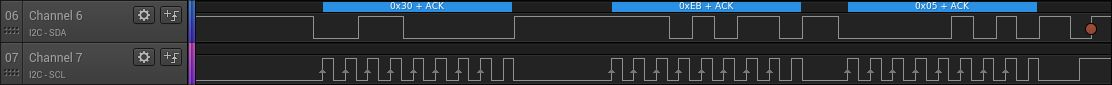
\includegraphics[trim={0cm 0cm 0cm 0cm},clip,scale=0.35]{Figures/trame.png}
    \decoRule
    \caption{Trame I2C} \label{fig:trame}
\end{figure} 

Sur le bus I2C, on a pu dénombrer 6 périphériques adressés 0x14, 0x15, 0xC8, 0xC9,
0x90 et 0x91. Nous nous sommes intéressé principalement à 0xC8 et 0xC9
vraisemblablement le SOM caméra et son interlocuteur (Openrex). On trouve dans les
communications qui lui sont adressées ce premier échange. dont nous ne sommes pas
sûr de l’interprétation.

\begin{itemize}
    \item[-] Setup Read to [0xC9] + ACK
    \item[-] 0x04 + NAK
    \item[-] Setup Write to [0xC8] + ACK
    \item[-] 0x00 + ACK
    \item[-] 0x01 + ACK
    \item[-] Setup Read to [0xC9] + NAK
\end{itemize}

Puis apparait le début de la structure de communication écrite dans le driver. Elle permet
de déverrouiller les configurations du fabricant mais n’est pas émise dans sa totalité et
s'interrompt au 3ème registre.

\begin{itemize}
    \item[-]Setup Write to [0xC8] + ACK
    \item[-]0x30 + ACK
    \item[-]0xEB + ACK
    \item[-]0x05 + ACK
    \item[-]Setup Write to [0xC8] + ACK
    \item[-]0x30 + ACK
    \item[-]0xEB + ACK
    \item[-]0x0C + ACK
    \item[-]Setup Write to [0xC8] + ACK
    \item[-]0x30 + ACK
    \item[-]0x0A + ACK
    \item[-]0xFF + ACK
    \item[-]Setup Write to [0xC8] + NAK
\end{itemize}